\section{Three 4-transpositions}

\begin{lemma}
  Let $\Gamma$ be a sggi of rank 4 on 11 points. If $\rho_1$, $\rho_2$ and $\rho_3$ are 4-transpositions and $\rho_0$ is a 2-transposition then the patterns formed by $\rho_1$ and $\rho_3$ edges are one alternating square, one double edge and two simple edges (one for each involution).\footnote{Extend this part}
\end{lemma}

\begin{proof}
  Suppose that there are two alternating squares. Those square can only be connected by $\rho_2$ simple edges. But those $\rho_2$ edges cannot be connected to other simple edge because all $\rho_1$ and $\rho_3$ have been used.

  \paragraph{}
  In fact, it is impossible to connect any $\rho_0$ edges to this graph. This edge cannot be connected directly because all $\rho_1$ edges have been used. It must be part of an alternating square. $[\rho_0, \rho_3]$ is impossible because a such square cannot be placed between to existing $\rho_3$ edge. The square must be $[\rho_0, \rho_2]$.

  \paragraph{}
  Thus a sequence of alternating square going from $[\rho_0, \rho_2]$ to $[\rho_1, \rho_3]$ must exists. Starting from $[\rho_1, \rho_3]$, the $\rho_3$ index must change in the next square because all of them have been used. But the same applies to $\rho_1$. This square cannot be part of a sequence therefore, there cannot be two alternating squares.

  \paragraph{}
  Suppose now that we have two double edges between $\rho_1$ and $\rho_3$. Those edges can be connected to the rest of the graph by a $\rho_2$ edge or be part of an alternating square.

  \paragraph{}
  At least one $\rho_1$ single edge is needed. Thus a single $\rho_3$ edge must also exists. This uses 10 vertices, therefore it cannot be two single $\rho_1$ edge.

  \paragraph{}
  Now let's proof that at least one alternating square must exists. Suppose that no alternating squares exists.

  \paragraph{}
  There are 2 $\rho_0$ edges. Those edges can be placed in alternating square, double edges or simple edges.

  \paragraph{}
  If it is placed in an alternating square it can be a component or just an additional edge.

  \paragraph{}
  If it just an additional edge, the other component must be $\rho_1$. And those edges cannot be doubled. Therefore there are 2 $\rho_1$ edges. At least one of them must therefore be part of an alternating square or a double edge. But the latter is impossible and therefore the former is mandatory.

  \paragraph{}
  If it is a component of a square, the other component must be $\rho_2$ or $\rho_3$. If it is $\rho_3$ it must be  adjacent to another square. It can be $[\rho_0, \rho_2]$ or $[\rho_1, \rho_3]$. The two cases are impossible.

  \paragraph{}
  The $\rho_0$ edges are not placed in an alternating square. Each must be connected by a $\rho_1$. An alternating square or a double edge is not possible. But that is a contradiction.
\end{proof}

\begin{theorem}
  All sggi of rank 4 on $A_{11}$ with three 4-transpositions are those displayed in appendix~\ref{rank4-3-4transpositions}
\end{theorem}

\begin{proof}
  Let, without loss of generality, $\rho_1$ and $\rho_3$ be 4-transposition.

  \begin{figure}[H]
    \begin{center}
      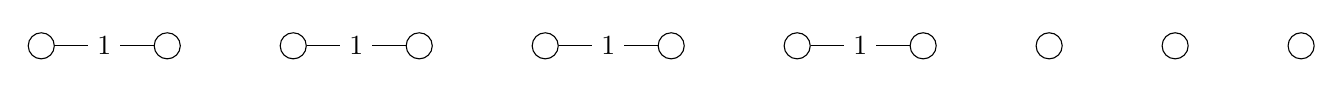
\begin{tikzpicture}[scale=.8]

        \begin{scope}[every node/.style={circle,draw}]
          \node (1)  at (0,0)  {};
          \node (2)  at (2,0)  {};
          \node (3)  at (4,0)  {};
          \node (4)  at (6,0)  {};
          \node (5)  at (8,0)  {};
          \node (6)  at (10,0)  {};
          \node (7)  at (12,0)  {};
          \node (8)  at (14,0)  {};
          \node (9)  at (16,0)  {};
          \node (10) at (18,0)  {};
          \node (11) at (20,0) {};
        \end{scope}

        \begin{scope}[every node/.style={fill=white}]

          \begin{scope}[every edge/.style={draw}]
            \path (1)  edge node {$1$} (2);
            \path (3)  edge node {$1$} (4);
            \path (5)  edge node {$1$} (6);
            \path (7)  edge node {$1$} (8);
          \end{scope}
        \end{scope}

      \end{tikzpicture}
      \caption{}
    \end{center}
  \end{figure}

  \paragraph{}By previous Lemma, the pattern between $\rho_1$ and $\rho_3$ is the following.


  \begin{figure}[H]
    \begin{center}
      \begin{tikzpicture}[scale=.8]

        \begin{scope}[every node/.style={circle,draw}]
          \node (1)  at (0,2)  {};
          \node (2)  at (0,0)  {};
          \node (3)  at (2,2)  {};
          \node (4)  at (2,0)  {};
          \node (5)  at (4,0)  {};
          \node (6)  at (6,0)  {};
          \node (7)  at (8,0)  {};
          \node (8)  at (10,0) {};
          \node (9)  at (12,0) {};
          \node (10) at (14,0) {};
          \node (11) at (16,0) {};
        \end{scope}

        \begin{scope}[every node/.style={fill=white}]

          \begin{scope}[every edge/.style={draw}]
            \path (1)  edge node {$1$} (2);
            \path (3)  edge node {$1$} (4);
            \path (5)  edge[bend right=30] node {$1$} (6);
            \path (7)  edge node {$1$} (8);
            \path (1)  edge node {$3$} (3);
            \path (2)  edge node {$3$} (4);
            \path (5)  edge[bend left=30] node {$3$} (6);
            \path (9)  edge node {$3$} (10);
          \end{scope}
        \end{scope}

      \end{tikzpicture}
      \caption{}
    \end{center}
  \end{figure}

  \paragraph{}
  Let's place the $\rho_0$ edges. We know by the proof of the previous lemma that one edge must be added to an alternating square. The other must be a single edge. This last edge must be connected by the single $\rho_1$ edge.

  \begin{figure}[H]
    \begin{center}
      \begin{tikzpicture}[scale=.8]

        \begin{scope}[every node/.style={circle,draw}]
          \node (1)  at (0,2)  {};
          \node (2)  at (0,0)  {};
          \node (3)  at (2,2)  {};
          \node (4)  at (2,0)  {};
          \node (5)  at (4,0)  {};
          \node (6)  at (6,0)  {};
          \node (7)  at (14,0)  {};
          \node (8)  at (12,0)  {};
          \node (9)  at (8,0)  {};
          \node (10) at (10,0)  {};
          \node (11) at (16,0) {};
        \end{scope}

        \begin{scope}[every node/.style={fill=white}]

          \begin{scope}[every edge/.style={draw}]
            \path (1)  edge[bend left=30] node {$0$} (3);
            \path (7)  edge node {$0$} (11);
            \path (1)  edge node {$1$} (2);
            \path (3)  edge node {$1$} (4);
            \path (5)  edge[bend left=30] node {$1$} (6);
            \path (7)  edge node {$1$} (8);
            \path (1)  edge[bend right=30] node {$3$} (3);
            \path (2)  edge node {$3$} (4);
            \path (5)  edge[bend right=30] node {$3$} (6);
            \path (9)  edge node {$3$} (10);
          \end{scope}
        \end{scope}

      \end{tikzpicture}
      \caption{}
    \end{center}
  \end{figure}

  \paragraph{}
  There are only 4 $\rho_2$ edges waiting to be placed. Three of them must link the components. The last one must double something. The only two possibilities: triple the double edge $(\rho_0, \rho_3)$ or double the other $\rho_0$.

  \paragraph{}
  If the single edge is double, the graph where the $\rho_1$ edge is removed is always this one:

  \begin{figure}[H]
    \begin{center}
      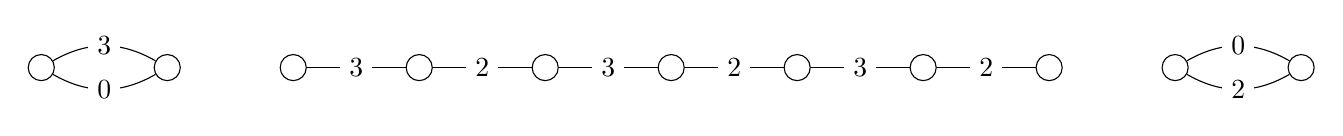
\begin{tikzpicture}[scale=.8]

        \begin{scope}[every node/.style={circle,draw}]
          \node (1)  at (-4,0)  {};
          \node (2)  at (-2,0)  {};
          \node (3)  at (14,0)  {};
          \node (4)  at (16,0) {};
          \node (5)  at (8,0)  {};
          \node (6)  at (10,0)  {};
          \node (7)  at (0,0)  {};
          \node (8)  at (2,0)  {};
          \node (9)  at (4,0)  {};
          \node (10) at (6,0)  {};
          \node (11) at (12,0)  {};
        \end{scope}

        \begin{scope}[every node/.style={fill=white}]

          \begin{scope}[every edge/.style={draw}]
            \path (1)  edge[bend right=30] node {$0$} (2);
            \path (3)  edge[bend left=30] node {$0$} (4);
            \path (3)  edge[bend right=30] node {$2$} (4);
            \path (5)  edge node {$2$} (10);
            \path (6)  edge node {$2$} (11);
            \path (8)  edge node {$2$} (9);
            \path (1)  edge[bend left=30] node {$3$} (2);
            \path (5)  edge node {$3$} (6);
            \path (7)  edge node {$3$} (8);
            \path (9)  edge node {$3$} (10);
          \end{scope}
        \end{scope}

      \end{tikzpicture}
      \caption{[1, 1029, 8827, 994]}
    \end{center}
  \end{figure}

  \paragraph{}
  But here it is clear that $\rho_0 = (\rho_2 \rho_3)^7$. Thus the last $\rho_2$ edge must triple to existing double edge.

  \paragraph{}
  The components can be link in a lot of different ways. The reader is advised to try to find all sggis and check that those displayed in appendix~\ref{rank4-3-4transpositions} are correct. Once more it can help to sort them by the length of the chain between the square and the double edge and then by the length of the chain between the double edge and the end of the graph.

\end{proof}

\begin{theorem}
  None of those graphs are C-groups.
\end{theorem}

\begin{proof}
  As for previous similar proof, only the summary is displayed and the details is left to the reader.

  \begin{table}[H]
    \centering
    \begin{tabular}{|c|c|c|c|c|c|c|}
      \hline
      Figure & $\Gamma_3$ & $\Gamma_0$ & $\Gamma_{0,3}$ & $\#\Gamma_{0,3}$ & $\Gamma_3 \cap \Gamma_0$ & $\#(\Gamma_3 \cap \Gamma_0)$ \\ \hline

      \ref{r4-5-1} & $S_7 : D_8$ & $A_{10}$ & $D_{42}$ & 42 & $\ge S_5$ & $\ge 120$ \\ \hline
      \ref{r4-5-2} & $A_{10}$ & $A_{10}$ & $D_{18}$ & 18 & $A_9$ & $181440$ \\ \hline
      \ref{r4-5-3} & $A_{10}$ & $A_{10}$ & $D_{18}$ & 18 & $A_9$ & $181440$ \\ \hline
      \ref{r4-5-4} & $S_7 : D_8$ & $A_{10}$ & $D_{42}$ & 42 & $\ge S_5$ & $\ge 120$ \\ \hline
      \ref{r4-5-5} & $A_5 : S_6$ & $A_{10}$ & $D_{10}$ & 10 & $\ge S_4$ & $\ge 24$ \\ \hline
      \ref{r4-5-6} & $A_8 : S_3$ & $A_{10}$ & $D_{42}$ & 42 & $\ge S_5$ & $\ge 120$ \\ \hline

    \end{tabular}
  \end{table}
\end{proof}
